\chapter{Design}

In this chapter, we properly introduce Psnodig and relevant design decisions behind the tool. We also describe the design behind the Gourmet programming language, as well the desicions behind the writers we landed on.

\section{Proposed Solution}

To solve the problem we are dealing with, we introduce Psnodig. We believe that Psnodig offers something unique in the context of this problem. Psnodig is a transpiler, first and foremost intended to convert executable programs to equivalent presentation-only programs. \\

We wish to alleviate common frustrations associated with pseudocode, like unbalanced parentheses, forgetting to consistently rename variables, issues related to performance and more. At the same time, we aim to preserve the good things that pseudocode let us have, like flexibility and abstraction, and using more precise mathematical notation. \\

The software discussed in Section 3.3 all do a very good job in their own right. The effort invested by developers, researchers and others involved is clearly reflected in both functionality and performance in each application. \\

However, the results they generate are sealed, and we have no choice but to accept whatever we receive. We believe there is more value in a tool that also lets us modify the final result, in case the translation from source code to PDF is ultimately too lossy. \\

Additionally, we believe these writers actually lie in the same sphere. Thus, it would make sense to gather and apply them in the same tool, rather than having to switch between different ones. Lastly, we see value in users adding their own parsers and code generators, to further increase the tool's usefulness. \\

As the programs discussed in Section 3.3.2 specialise in flowchart generation, the DSLs are not actually executable. We believe that this is something that could be of tremendous use, and have therefore incorporated an interpreter that works on the internal representation of Psnodig. To the best of our knowledge, a tool which combines these exact devices does not currently exist.

\section{Psnodig}

At its core, Psnodig is really just an intermediate representation through an AST. As such, it does not provide a lot of functionality on its own. It is first when we add parsers and writers that it shows its usefulness. Currently, it boasts one parser and four writers, as portrayed in \Cref{The parsers and writers of Psnodig.}, depicting the parsers on the left and writers on the right. \\

\begin{figure}[ht]
    \centering
    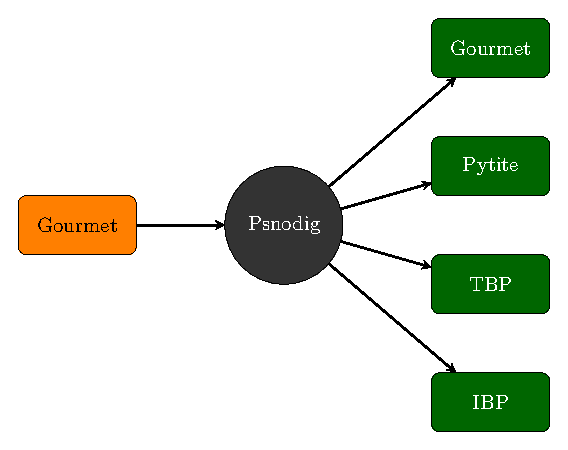
\includegraphics[scale=0.7]{assets/chapter4/Psnodig.pdf}
    \caption{The parsers and writers of Psnodig.}
    \label{The parsers and writers of Psnodig.}
\end{figure}

Since we are free to add parsers and writers at will, only our imagination (and programming abilities) can limit what we use it to convert. However, it is first and foremost intended as a tool for converting executable source programs to a presentation-only target programs. \\

Psnodig's transpilation flow is as follows: source programs are parsed to an internal, intermediate representation. Later, this representation is used to convert the original program further to a new target program. This means that a source program written in different languages can produce the same target program, given that their ASTs are identical. \\

Psnodig also comes with an interpreter, which works on the internal representation. This means that we can add parsers and run the code, without also having to write an interpreter or compiler. \\

All of this leads to a feeling of predictability: We write our source code in an available language. Then we use the interpreter to test it, until we are satisfied with the results. Now we are able to transpile it to TBP and IBP through the command line, rather than having to reconstruct it all manually. \\

Currently, Psnodig offers multiple command line arguments. By running \texttt{psnodig help} in the command line, we are presented with \Cref{psnodigCMDoptions}, which discloses our remaining options. \\

\begin{lstlisting}[caption={The command line options for Psnodig, presented by running \texttt{psnodig help} in the terminal.}, captionpos=b, label={psnodigCMDoptions}]
Psnodig - a general transpiler with options for pseudocode and flowcharts.

Available options:

<psnodig program>          : Parses the program and runs it
                             through the interpreter.

<psnodig ast program>      : Prints the program's AST to the
                             terminal.

<psnodig tbp program>      : Transpiles the program to TBP in
                             LaTeX.
<psnodig tbp pdf program>  : The same as above, but also
                             compiles the LaTeX file to a PDF.

<psnodig ibp program>      : Transpiles the program to IBP in
                             LaTeX.
<psnodig ibp pdf program>  : The same as above, but also
                             compiles the LaTeX file to a PDF.

<psnodig gourmet program>  : Transpiles the program to the
                             equivalent in Gourmet.
<psnodig Python program>   : Transpiles the program to the
                             equivalent in Python.

<psnodig help>             : Brings you back here!
\end{lstlisting}

% \texttt{psnodig program}, which parses a program and runs it through the interpreter. If our program contains any reachable print-statements, their arguments will be printed back to the command line. \\

% \texttt{psnodig tbp program}, which parses the program and produces a LaTeX file containing the program's TBP version. We can also add a flag \texttt{pdf} after \texttt{tbp} to get a PDF of the compiled LaTeX file. \\

% \texttt{psnodig ibp program}, which parses the program and produces a LaTeX file containing the program's IBP version. We can also add a flag \texttt{pdf} after \texttt{ibp} to get a PDF of the compiled LaTeX file. \\

% \texttt{psnodig gourmet program}, which parses a source program to an equivalent program in Gourmet syntax. As we only have a parser for Gourmet, converting Gourmet programs back to themselves has been a way to test Psnodig's consistency. \\

% \texttt{psnodig Python program}, which transpiles a source program to an equivalent program in Python syntax. \\

% \texttt{psnodig ast program}, which prints the program's AST to the terminal, given that the program is syntactically correct. This can be a nice way to debug programs, and get a better understanding of how our parsers actually parse our programs. \\

% \texttt{psnodig help}, which yields all the legal commands, and what they provide, in the command line.

\subsection{Syntax}

Psnodig's syntax is located at \Cref{Psnodig's data types in Haskell.}, in the form of Haskell data types. \\

The entry point of a Psnodig program is \texttt{Program}. Since all of its symbols are optional, a minimal working example is actually an empty file. This flexibility allows our parsers and writers to utilise just as much, or as little, of the Psnodig syntax as we wish. \\

Most of the syntax resembles the syntax of common programming languages. However, there are two statements that have been introduced specifically for Psnodig's real use case: \texttt{Hash statements} and \texttt{Annotation statements}. \\

\textbf{Hash statements} are picked up by the parser and intended to be interpreted, but ignored by writers. This lets us abstract away things that we deem to be obvious to our audience. It could also be things that have already been stated elsewhere, but still need to be parsed for our programs to run. The name derives from how we can write single line comments in Python with a hash symbol. \\

A common use case of this is how a lower case \texttt{n} is often used to denote amounts in TBP. By using a hash statement, we avoid including superflous length-function calls in cases where it is obvious what \texttt{n} symbolises. However, this will never be obvious to the interpreter, and thus we still have to include it in our source programs somehow. \\

\Cref{An AST of a hash statement.} shows an AST of a hash statement. An example of a hash statement in action can be seen in \Cref{hashStmtInAction}. \\

\begin{figure}[ht!]
    \Tree [.\texttt{Hash statement} \texttt{``\#''} \textit{statement} ]
    \caption{An AST of a hash statement.}
    \label{An AST of a hash statement.}
\end{figure}

\textbf{Annotation statements} are statements that allow us to add an extra layer of abstraction to our output targets. The first string is what is transpiled, without any conversion, whilst the list of statements is reserved for the interpreter. \\

A common use case of this is when we wish to swap two elements in a list. In many programming languages, when swapping two elements \texttt{a} and \texttt{b}, we have to assign \texttt{a} to a temporary variable, then assign \texttt{a} to \texttt{b}, before we can finally assign \texttt{b} to that temporary variable. These three implementation-specific lines could easily be abstracted with \texttt{swap a and b}. \\

We can also leave the first value of an Annotation statement to be an empty string. This means that the statement list will be interpreted, but nothing will show in the TBP or IBP versions. This also means that Annotation statements to some extend are supersets of Hash statements, offering the same functionality, but allowing more than statement at the time. \\

Likewise, the second value of an Annotation statement can be left empty. This allows us to explain things solely with natural language. \Cref{An AST of an annotation statement.} shows an AST of an annotation statement. An example of an annotation statement in action can be seen in \Cref{antStmtInAction}. \\

\begin{figure}[ht!]
    \Tree [.\texttt{Annotation statement} string \texttt{[}\textit{statement}\texttt{]} ]
    \caption{An AST of an annotation statement.}
    \label{An AST of an annotation statement.}
\end{figure}

These two statements are particularly useful when a piece of code is not crucial to the program's logic, or when the code is very implementation specific.

\subsection{Interpreter}

A big selling point of Psnodig is that in addition to being a transpiler, we also provide an interpreter which works on the internal representation. For a program to be transpiled, it only needs to be syntactically correct. However, this does not guarantee that the program works as intend. Thus, Psnodig provides users with the ability to test their programs before they are transpiled and later presented, which can be crucial. \\

Take the program presented in \Cref{A syntactically correct program with a subtle logical error.} as an example. The function \\ \texttt{printEvenNumbers} takes two arguments: a list of numbers and the list's length. Then we iterate through this range, and proceed to print every number in the list that is even. However, we check for evenness by doing \texttt{if i \% 2 == 0}, when really we intend to do \texttt{if numbers[i] \% 2 == 0}. The difference is subtle, but by running the program we quickly realise the error when the screen displays 47, 79 and 93 rather than 46 and 22. \\

\begin{lstlisting}[caption={A syntactically correct Gourmet program with a subtle logical error.}, captionpos=b, label={A syntactically correct program with a subtle logical error.}]
func printEvenNumbers(numbers list, length int) {
    for i := 0, length-1 {
        if i % 2 == 0 {
            print(numbers[i])
        }
    }
    return 1
}

printEvenNumbers([47, 46, 79, 22, 93], 5)
\end{lstlisting}

As seen from the syntax in \Cref{Psnodig's data types in Haskell.}, Psnodig programs consist of four parts: An optional program description, a list of struct declarations (which can be empty), a list of function declarations (which can also be empty), and lastly, an optional function call. The function call works as the interpreter's entry point, but is ignored by the both pseudocode writers.

\subsubsection{Scope}

Psnodig works with both a global and a local scope. All structs and functions are global, and can be accessed from within any function. This means that, among other things, functions can be mutually recursive. Variables, on the other hand, are strictly local, and a variable declared in function \texttt{f} cannot be accessed in function \texttt{g}, unless passed as an argument. \\

\Cref{Gourmet program which provokes a runtime error.} and \Cref{Gourmet code without error.} both show syntactically correct programs. However, running the former will yield a runtime error, because \texttt{n} is not available in the scope of \texttt{g}. The latter program will run smoothly, as we pass the variable as an argument to \texttt{g}, which excitedly returns the variable straight back. \\

\begin{minipage}{.45\textwidth}
\begin{lstlisting}[caption={Gourmet program which provokes a runtime error.}, captionpos=b, label={Gourmet program which provokes a runtime error.}]
func f() {
    n := 5
    return g()
}

func g() {
    return n
}

f()
\end{lstlisting}
\end{minipage}\hfill
\begin{minipage}{.45\textwidth}
\begin{lstlisting}[caption={Gourmet program that will run uninterrupted.}, captionpos=b, label={Gourmet code without error.}]
func f() {
    n := 5
    return g(n)
}

func g(n int) {
    return n
}

f()
\end{lstlisting}
\end{minipage}

Psnodig supports nested scopes as indicated by the \texttt{For String Expression Expression [Statement]} value within the \texttt{Statement} type in \Cref{Psnodig's data types in Haskell.}. The two \texttt{Expression} data types define a range, whilst the \texttt{String} data type serves as an identifier that binds to all numbers within this specified range (inclusive). \\

The statements are then executed repeatedly for each value in this range, with the identifier reflecting the current value on each iteration. Once the loop terminates, the identifier is automatically unbound, and no longer exists in any context.

\subsubsection{Iterating Expressions}

\Cref{Psnodig's data types in Haskell.} shows that Psnodig prohibits two types of \texttt{For}-loops. \texttt{For String Expression [Statement]} is discused in the previous subsection, but we also entertain \texttt{ForEach String Expression [Statement]}. This is intended to mimic standard \texttt{For each}-loops found in languages like Go and Python. \\

One could say that it is too expressive, technically allowing iteration of non-iterables like arithmetic expressions. However, since all iterables also fall under the \texttt{Expression} type, we allow it syntactically, and instead deal with it on the interpreter side.

\subsubsection{Built-in Functions}

The interpreter provides several built-in functions, which are also found in many programming languages. They are also reflected in the TBP writer. If a function call fails, e.g. due to wrong number of arguments provided, or arguments having the wrong type, the program will stop and the user will receive an explanatory error message. \\

\textbf{print($x_{1}$, $..$, $x_{n}$)}, which takes $n \in \mathbb{N}$ arguments. The arguments must be of type \texttt{Expression}. Each argument is converted to a string and concatenated, separated by a space, before they are printed to the terminal. The function returns the number of arguments passed to it. \\

\textbf{length($x$)}, which takes one argument. The argument must be of type \texttt{Text}, \texttt{List}, \texttt{HashSet}, or \texttt{HashMap} (presented in \Cref{Psnodig's data types in Haskell.}). The function returns the length of its argument: Number of characters in the text, number of elements in the list or hashset, or number of mappings in the hashmap. \\

\textbf{ceil($x$)}, which takes one number $x \in \mathbb{Q}$ as argument. The return value will be rounded up to the nearest $n \in \mathbb{N}$. \\

\textbf{floor($x$)}, which takes one number $x \in \mathbb{Q}$ as argument. The return value will be rounded down to the nearest $n \in \mathbb{N}$. \\

\textbf{max($x_{1}$, $..$, $x_{n}$)}, which takes $n \in \mathbb{N}_{>0}$ arguments. The arguments themselves must be an $x \in \mathbb{Q}$. The return value will be the largest value amongst the arguments. \\

\textbf{min($x_{1}$, $..$, $x_{n}$)}, which takes $n \in \mathbb{N}_{>0}$ arguments. The arguments themselves must be an $x \in \mathbb{Q}$. The return value will be the smallest value amongst the arguments. \\

\textbf{append($x$, $xs$)}, which takes two arguments. The first argument must be an \texttt{Expression}, and the second argument must be a \texttt{List}. The function will append $x$ to the end of $xs$, thus modifying the list locally. The function returns 1 upon success. \\

\textbf{add($x$, $hs$)}, which takes two arguments: an \texttt{Expression} $x$ and a \texttt{HashSet} $hs$. It adds the former to the latter. The function returns 1 upon success. \\

\textbf{add($k$, $v$, $hm$)} is an overloaded version of \textbf{add}, this time taking three arguments: An \texttt{Expression} $k$, an \texttt{Expression} $v$, and a \texttt{HashMap} $hm$. It maps $k$ to $v$, and adds the mapping to $hm$. This version of the function also returns 1 upon success. \\

\textbf{get($k$, $hm$)}, which takes two arguments, an \texttt{Expression} $k$ and a \texttt{HashMap} $hm$. If $k$ is a key in $hm$, the function returns the value $v$ that $k$ maps to in $hm$. \\

\textbf{in($x$, $xs$)}, which takes two arguments, an \texttt{Expression} $x$ and either a \texttt{List}, a \texttt{HashSet}, or a \texttt{HashMap}. The function will check if $x$ exists in $xs$, and return the appropriate boolean. \\

\textbf{pop($x$)}, which takes one argument, a non-empty \texttt{List} $x$. If the list is not empty, the function will modify $x$ by removing $v$, before subsequently returning $v$. \\

\textbf{toString($x$)}, which takes one argument, an \texttt{Expression} $x$. It returns the string version of $x$. Base expressions and lists will look identical, whilst hashset, hashmap and struct expressions vary. \\

Hashsets are printed on the form \texttt{(expr$_1$, .., expr$_n$)}, hashmaps are printed on the form \texttt{\{key$_1$:value$_1$, .., key$_n$:value$_n$\}}, and structs are printed on the form \texttt{field$_1$:value$_1$, field$_n$:value$_n$}. Nested structs are enclosed in parentheses.

\section{Gourmet}

To make sure Psnodig works at all, we depend on having at least one input target and one output target. When it comes to input language, we have two plausible alternatives: Use an existing programming language, or design a new one. We have opted for the latter. \\

In the context of Psnodig, we just need to build a parser that can translate programs in the source language to the intermediate representation. There are several reasons as to why designing a new language for the purpose of proof of concept is a good choice. \\

For one, it demonstrates the general effort to add a new input target for Psnodig. This can motivate others to add their own language, or even write parsers for existing languages. \\

Another reason is that selecting a single programming language to encompass all needs is not feasible. For instance, the largest university in southern Norway uses Python for its introductory programming course~\cite{pythonHosUIO}, whilst the largest university in northern Norway prefers C~\cite{cHosUIT}. The largest university in Greece sticks to Java~\cite{javaIHellas}, and Harvard's renowned CS50 course introduces students to both JavaScript and SQL~\cite{javaScriptOgSQLhosHarvard}. \\

What the languages of computer science introductory courses do have in common, is that they tend to be within the imperative paradigm of computer programming. Therefore, we aimed to stay in the same sphere, and Gourmet's syntax is mainly inspired by imperative programming languages like Go and Python. In fact, Gourmet started out as a pure subset of the former, hence its name: A gourmet portion of Go.

\subsection{Lexical Aspects}

Before we reveal Gourmet's grammar, we believe it is valuable to walk thorugh important lexical aspects like keywords, comments and whitespace. These are handled by the lexer, which is presented in its entirety in \Cref{The Gourmet lexer.}.

\subsubsection{Identifiers and Keywords}

An identifier in Gourmet is used to reference either a struct, function or variable. Identifiers are restricted to begin with a letter, followed by an arbitrary number of letters, numbers, and single quotes. \texttt{variable}, \texttt{var1able’} and \texttt{g0urmetVar1able''’'} are all valid Gourmet identifiers, whilst \texttt{1variable} and \texttt{'variable} are both not. Additionally, an identifier cannot shadow already existing keywords. \\

In total, there are 14 keywords in Gourmet: \texttt{while}, \texttt{if}, \texttt{func}, \texttt{true}, \texttt{false}, \texttt{return}, \texttt{else}, \texttt{for}, \texttt{break}, \texttt{continue}, \texttt{struct}, \texttt{not}, \texttt{map} and \texttt{set}. These keywords are also reserved, which means that we cannot define identifiers like \texttt{while} and \texttt{func}. \\

Gourmet allows us to define functions that shadow the built-in functions of Psnodig, however the interpreter will always prefer the built-in ones. While we cannot write and run a function called \texttt{print}, we can always define a function \texttt{print’} or \texttt{print1}, which will be handled just like any other function we define ourselves.

\subsubsection{Comments}

As there are no data types for comments in Psnodig, they must be handled individually by each lexer. Gourmet supports both single- and multi-line comments, identical to the ones found in most C-like languages like C itself, Go, Java, and more. \\

Single-line comments begin with a double forward slash \textbf{//}, and extend to the end of that line. Multi-line comments start with a forward slash and a star \textbf{/*}, and end with a star and a forward slash \textbf{*/}. Multi-line comments cannot be nested, which means that the first \textbf{*/} after a \textbf{/*} will end that comment, no matter how many \textbf{/*} preceeds it. A practical example of how they work can be seen in \Cref{Example of legal and illegal comments in Gourmet.}. \\

\begin{lstlisting}[caption={Example of legal and illegal comments in a Gourmet program.}, captionpos=b, label={Example of legal and illegal comments in Gourmet.}]
func f() {
    // This is a single-line comment.

    /* This is a

       multi-line
       comment.
       */

    /* However, our lexer
    does not allow
        /* nested
        multi-line
    */  comments.
    */
}
\end{lstlisting}

\subsubsection{Whitespace}

Whitespace can be defined as spaces, newlines and tabs. Gourmet does not differentiate between any of them, and we can use them in our programs exactly how we wish. \\

\Cref{f with a standard amount of whitespace.}, \Cref{f with a lot of whitespace.} and \Cref{f with no whitespace.} show three identical programs, besides the use of whitespace. We have a function \texttt{f}, which defines a variable \texttt{a} and returns it. All three programs will be parsed successfully, and have the same internal representation in Psnodig. \\

\begin{lstlisting}[caption={A Gourmet program with a standard amount of whitespace.}, captionpos=b, label={f with a standard amount of whitespace.}]
func f() {
    a := [1, 2]
    return a
}
\end{lstlisting}

\begin{lstlisting}[caption={A Gourmet program with a lot of whitespace.}, captionpos=b, label={f with a lot of whitespace.}]
func f()
{
    a       :=
        [1   ,   2]
    return
    a
                }
\end{lstlisting}

\begin{lstlisting}[caption={A Gourmet program with no whitespace.}, captionpos=b, label={f with no whitespace.}]
funcf(){a:=[1,2]returna}
\end{lstlisting}

\subsection{Types}

Gourmet is dynamically typed, which means that we do not have to specify the type of variables and return type of functions. In fact, Gourmet does not even \textit{let} us. When defining structs and function arguments, however, we have to provide type hints on the form \texttt{name type}. \\

The reason behind this choice is solely to improve code readability. When defining a variable, the value will be clearly present on the right hand side. When working with function arguments, however, we can never be entirely sure what the caller may pass. With type hints, at least we have a grasp of the arguments' intended use.\footnote{This way of employing type hints is inspired by other dynamically typed languages like Python and PHP.} \\

However, any value evaluated at runtime will inherently have one of five base types:  \texttt{Boolean}, \texttt{Number}, \texttt{Decimal}, \texttt{Text}, and \texttt{Nil}. A boolean value is either true or false, a number value is an  $n \in \mathbb{N}$, a decimal value is a $q \in \mathbb{Q}$, and a text value is an arbitrary combination of UTF-8 characters within a pair of double quotes. \texttt{Nil} indicates the absence of a value, and often serves as a placeholder. \\

Essentially, types associate data values into classes and provide rules for how these classes should interact. Sometimes, the base types Gourmet offers might not suffice. For this reason, we can create our own types through \texttt{structs}. Structs in Gourmet work exactly the way they do in languages like C and Go, containing instance variables, but no methods or constructors, contrary to languages like Python and Java. \\

\Cref{Gourmet Tree} shows how we can create a struct for modelling a Tree data structure, and \Cref{A function to initialise three tree structs and return the last one.} shows how we can later initialise a variable to have a Tree value. \\

\begin{lstlisting}[caption={A Gourmet struct Tree, with instance variables \texttt{value}, \texttt{left} and \texttt{right}.}, captionpos=b, label={Gourmet Tree}]
struct Tree {
    value int,
    left Tree,
    right Tree
}
\end{lstlisting}

\begin{lstlisting}[caption={A function to initialise three Tree structs and return the last one.},captionpos=b, label={A function to initialise three tree structs and return the last one.}]
func f() {
    tree := struct Tree(10, nil, nil)
    tree' := struct Tree(20, nil, nil)
    tree'' := struct Tree(15, tree, tree')
    return tree''
}
\end{lstlisting}

\subsection{Evaluation Strategy}

The Psnodig interpreter operates with a strict call-by-value evaluation strategy, just like the Pascal programming language.\footnote{\url{https://www.freepascal.org/docs-html/ref/refsu68.html}} When we pass lists or structs as arguments to a function, it has the capability to modify indexes and fields. However, these changes remain local to the function's scope and do not affect the caller's original data structure.

\subsection{Syntax}

\subsubsection{Grammar}

We present Gourmet's EBNF grammar in \Cref{The EBNF grammar of the Gourmet programming language.}. EBNF, short for Extended Backus-Naur form, is a simple, precise and sufficiently powerful notation to formally describe the syntax of a programming language~\cite{whatIsEBNF}. We could have opted for the original BNF notation, but EBNF allows us to present it more suffinctly. \\

We use a few meta symbols to help describe the grammar:

\begin{itemize}
    \item $\Leftarrow$ indicates the application of a rule. For instance, \texttt{X $\Leftarrow$ Y} means that \texttt{X} shall be substituted with \texttt{Y}.
    \item \texttt{\{ ... \}} indicates the repetition of 0 or more times (much like the reflexive arrow in \Cref{An example finite state automata.}).
    \item  \texttt{[ ... ]} indicates binary presentness. The content inside the square brackets is either present or it is not.
    \item \texttt{|} indicates disjunction, like we saw in Section 2.2.1.
    \item \texttt{" ... "} indicates a terminal: a Gourmet keyword without production rules.
\end{itemize}

Non-terminals are symbols that can be substituted. All the symbols on the left side of the arrows are non-terminals, and they often appear on the right side too. We write them in uppercase. Additionally, there are seven terminals written in uppercase, appearing solely on the right side of the arrows. They are \texttt{NAME}, \texttt{STRING}, \texttt{TEXT}, \texttt{INTEGER}, \texttt{DECIMAL}, \texttt{BOOLEAN}, and \texttt{NIL}. \\

\texttt{NAME} works as a placeholder for an identifier, e.g. the name of a function. \texttt{TEXT} is any combination of UTF-8 characters. It is used to provide program descriptions, and to serve as the first value of an Annotation statement. \texttt{STRING} is similar to \texttt{TEXT}, but requires the character sequence to be wrapped in double quotes. \texttt{INTEGER} is any $n \in \mathbb{N}$. \texttt{DECIMAL} is any $q \in \mathbb{Q}$. \texttt{BOOLEAN} is a $b \in \{\top, \bot \}$. Lastly, \texttt{NIL} is meant to indicate the absence of a value. \\

\begin{lstlisting}[caption={Gourmet's grammar in EBNF notation.}, captionpos=b, label={The EBNF grammar of the Gourmet programming language.}]
PROGRAM            $\Leftarrow$ [ PROGRAMDESCRIPTION ] { STRUCTDECL }
                      { FUNCTIONDECL } [ FUNCTIONCALL ]

PROGRAMDESCRIPTION $\Leftarrow$ "?" TEXT "?" "!" TEXT "!"

STRUCTDECL         $\Leftarrow$ "struct" NAME "{" { ARGUMENT } "}"

FUNCTION           $\Leftarrow$ "func" NAME "(" [ ARGUMENT { ","
                      ARGUMENT } ] ")" "{" { STATEMENT } "}"

ARGUMENT           $\Leftarrow$ NAME NAME

STATEMENT          $\Leftarrow$ "break" | "continue" | ANNOTATIONSTMT
                      | "#" STATEMENT | ASSIGNMENT | WHILE
                      | FOREACH | FOR | IF
                      | "return" EXPRESSION | FUNCTIONCALL


ASSIGNMENT         $\Leftarrow$ ASSIGNMENTTARGET ":=" ASSIGNMENTVALUE

LOOP               $\Leftarrow$ "while" EXPRESSION "{" { STATEMENT } "}"

IF                 $\Leftarrow$ "if" EXPRESSION "{" { STATEMENT } "}"
                      [ ELSE ]

FOREACH            $\Leftarrow$ "for" NAME ":=" EXPRESSION "{"
                      { STATEMENT } "}"

FOR                $\Leftarrow$ "for" NAME ":=" EXPRESSION ","
                      EXPRESSION "{" { STATEMENT } "}"

FUNCTIONCALL       $\Leftarrow$ NAME "(" EXPLIST ")"

ANNOTATIONSTMT     $\Leftarrow$ "@" "{" TEXT "}" "{" { STATEMENT } "}"

ASSIGNMENTTARGET   $\Leftarrow$ NAME | LISTINDEX | STRUCTFIELD

ASSIGNMENTVALUE    $\Leftarrow$ EXPRESSION | STRUCT

ELSE               $\Leftarrow$ "else" IF | "else" "{" { STATEMENT } "}"

EXPRESSION         $\Leftarrow$ VALUE | NAME | LISTINDEX
                      | EXPRESSION OPERATOR EXPRESSION
                      | FUNCTIONCALL | "not" EXPRESSION
                      | STRUCT | STRUCTFIELD

LISTINDEX          $\Leftarrow$ NAME "[" EXPRESSION "]" { "["
                      EXPRESSION "]" }

OPERATOR           $\Leftarrow$ "+" | "-" | "*" | "/" | "<" | "<="
                      | ">" | ">=" | "==" | "!=" | "&&"
                      | "||" | "%"

STRUCT             $\Leftarrow$ NAME "(" EXPLIST ")"

STRUCTFIELD        $\Leftarrow$ EXPRESSION "." EXPRESSION

VALUE              $\Leftarrow$ "map" "{" [ PAIR { "," PAIR } ] "}"
                      | "set" "{" EXPLIST "}" | "nil"
                      | "true" | "false" | DECIMAL
                      | NUMBER | STRING | "[" EXPLIST "]"

PAIR               $\Leftarrow$ EXPRESSION ":" EXPRESSION

EXPLIST            $\Leftarrow$ [ EXPRESSION { "," EXPRESSION } ]
\end{lstlisting}

\forsup{Note: Håndterer expressions på en mye mer rotete måte enn det jeg viser til over. Har LL-parsing å gjøre. Skal finpusse det og endre den biten her og :)}

\subsubsection{Precedence and Associativity}

The precedence of Gourmet operators is ranked in the following order, from highest to lowest:

\begin{enumerate}
    \item $*$, $/$ and $\%$
    \item $+$ and $-$
    \item $<$, $<=$, $>$ and $>=$
    \item $==$ and $!=$
    \item $\&\&$ and $||$
    \item $.$
    \item not
\end{enumerate}

This means that if we wish to calculate the sum of the tree values from Listing 4.9, we cannot write \texttt{tree.value + tree'.value + tree''.value}, because the parser will parse \texttt{p.(value + p').(value + p'').value}. Therefore, we have to include parantheses to make \texttt{(tree.value) + (tree'.value) + (tree''.value)}. \\

All operations are left-associative.

\subsubsection{Compatibility with Psnodig}

An important part of being compatible with Psnodig, is handling hash- and annotation statements. Since Gourmet is developed with Psnodig in mind, it was natural to fit them in. \Cref{hashStmtInAction} shows a program with a hash statement, we use it to assign the length of a list to a variable. \Cref{antStmtInAction} shows a program with an annotation statement, where we use it to abstract swapping to variables in a list. \\

\begin{lstlisting}[caption={A Gourmet program with a hash statement}, captionpos=b, label={hashStmtInAction}]
func f(a: list) {
    # n := length(a)
    for i := 0, n {
        print(a[i])
    }
}
\end{lstlisting}

\begin{lstlisting}[caption={A Gourmet program with an annotation statement}, captionpos=b, label={antStmtInAction}]
func f(a: list) {
    if length(a) > 1 {
        @{swap a[0] and a[1]}{
            tmp := a[0]
            a[0] := a[1]
            a[1] := tmp
        }
    }
}
\end{lstlisting}

\subsection{Gourmet Writer}

In addition to having an input language, we need an output language to show that Psnodig works as intended. The output language could be just about anything, but since we designed a parser for Gourmet, we figured it would be interesting to also have a writer. \\

By having both a parser and a writer for the same language, we are able to test Psnodig's consistency. Since the languages are the same, we should be able to have a lossless conversion back and forth. Psnodig does not take formatting into consideration, so we might experience a difference in whitespace. However, as discussed in Section 4.3.1.3, whitespace cannot alter a Gourmet program's semantics, so this is not a problem. \\

Additionally, since Gourmet boasts most of the characteristics of other dynamically typed languages, the writer serves as a pointer to how much effort it might take to write a parser for another dynamically typed programming language, like Python or Ruby.

\section{Python Writer}

As mentioned in Section 4.3, Gourmet's syntax is mainly inspired by Go and Python. As they are far richer languages, and Gourmet almost resembles a subset of Go, we decided to create an additional writer which converts ASTs to Python-like syntax.

The Gourmet and Python writers are very similar, only with a few notable differences, like \texttt{=} over \texttt{:=} for assignment, and colons over curly brackets. The biggest difference, however, is handling structs, as Python does not have them. Instead, they have \textit{classes}. \Cref{The Python equivalent of an empty struct in Gourmet.} shows how we translate an empty struct \texttt{struct Struct\{\}} into a class. \\

\begin{lstlisting}[caption={The Python equivalent of an empty struct in Gourmet.}, captionpos=b, label={The Python equivalent of an empty struct in Gourmet.}]
class Struct:
    def __init__(self):
        pass
\end{lstlisting}

Additionally, while Gourmet allows all type hints, Python only allows a few (without importing external libraries). Therefore, if a type hint is not \texttt{int}, \texttt{float}, \texttt{double}, \texttt{str}, \texttt{boolean}, or \texttt{nil}, they are simply removed from the final Python version. \\

Most of Psnodig's built-in functions have equivalents in Python, but not all. For instance, to use \texttt{min} and \texttt{max}, we would have to install the \texttt{math} package. Other than those, we translate \texttt{length} to \texttt{len}, \texttt{get(key, hashmap)} to \texttt{hashmap[key]} etc., given that the correct number of arguments is provided. \\

Python does not inherently have hash- and annotation statements. However, while these are statements that are intended to be hidden during presentation, they are essential to a program's runtime. Therefore, we have decided to convert them to regular statements in Python, also ignoring the first argument of annotation statements. \\

Lastly, for descriptions of input and output, we have decided to put them at the start of the file as block comments. \Cref{gourmetSquareVariable} shows a program in Gourmet, and \Cref{PythonResult} shows the transpiled version in Python. \\

\begin{lstlisting}[caption={A Gourmet function where an input variable gets squared and returned.}, captionpos=b, label={gourmetSquareVariable}]
? An integer x ?
! The integer x squared !

func f(x int) {
    return x * x
}
\end{lstlisting}

\begin{lstlisting}[caption={The result of transpiling \Cref{gourmetSquareVariable} to Python with Psnodig}, captionpos=b, label={PythonResult}]
# Input: An integer x 
# Output: The integer x squared 

def f(x: int):
    return x * x
\end{lstlisting}

\section{Pseudocode Writer}

An important part of Psnodig is the ability to convert source code to equivalents on a different abstraction level. One of our writers transpile internal representations TBP in LaTeX.\footnote{The writer can be found here: link} As previously stated, we are not attempting to create a ground truth for pseudocode. Therefore, we have chosen to work with an already-established package for writing pseudocode like Algorithm2e. \\

Structs and the initial function call are not converted to pseudocode. For one, we believe that function calls are rarely cruical to the algorithm itself, and structs will always be implementation specific. The second reason is that there does not seem to be an obvious way of transpiling them anyway, in a way that adds particular value.

\subsection{Compatibility with Psnodig}

As already mentioned in Section 4.2.2.3, all Psnodig library functions are taken into consideration by the TBP writer. The function call \texttt{ceil(decimal)} is transpiled with mathematical symbols to $\lceil decimal \rceil$. The function call \texttt{append(x, xs)} is transpiled to the natural language description \texttt{append x to xs}. \\

Mathematical expressions are also taken into account. For instance, the value \texttt{BinaryExp Division (Constant (Number 2)) (Constant (Number 1))} will show $\frac{2}{1}$, rather than something like \texttt{2/1}. Similarly, an expression with multiplication will be displayed as \texttt{m $\cdot$ n} rather than \texttt{m * n}. To work with mathematical symbols in LaTeX we use the packages \texttt{amsmath} and \texttt{commath}. They are always included, regardless of the rest of the program. \\

We also declare some macros to match the syntax of Psnodig. Before our programs are transpiled to TBP, we scan it for keywords, which are then reflected the LaTeX file. If our program contains code like \texttt{v := false}, the LaTeX file will include \texttt{\textbackslash SetKw\{False\}\{false\}}, and we will apply \texttt{\textbackslash KwFalse} rather than just ``false''.

\subsection{Output}

If we run \texttt{psnodig tbp program} in our command line, and the program is syntactically correct, we receive a corresponding LaTeX file. If we add the \texttt{pdf} flag we also get a PDF of the compiled LaTeX file. \\

Just like the Gourmet writer, the TBP writer is not able to take the original source code's formatting into account. This means that a program like the one shown in \Cref{Gourmet f} will be transpiled to the one shown in \Cref{How Psnodig transpiles the program from} rather than the one shown in \Cref{Alternative version of f in LaTeX with Algorithm2e.}. \\

\begin{lstlisting}[caption={A Gourmet function which declares a variable and returns it.}, captionpos=b, label={Gourmet f}]
func f(){v:=5 returnv}
\end{lstlisting}

\begin{lstlisting}[caption={How Psnodig transpiles the program from \Cref{Gourmet f}.}, captionpos=b, label={How Psnodig transpiles the program from}]
\proc{$\f()$}{
    $\texttt{v} \gets 5$ \;
    \Return $v$ \;
}
\end{lstlisting}

\begin{lstlisting}[caption={Alternative version of f in LaTeX with Algorithm2e.}, captionpos=b, label={Alternative version of f in LaTeX with Algorithm2e.}]
\proc{$\f()$}{$\texttt{v}\gets5$\;\Return$v$;}
\end{lstlisting}

Even though the compiled versions produce the same PDF, we believe the curated amount of whitespace increases the maintainability of the LaTeX document, in case we wish to tweak it manually after transpilation. All transpiled documents will include \texttt{\textbackslash SetKwProg\{proc\}\{Procedure\}\{\}\{\}}, and the one transpiling \Cref{Gourmet f} will also have \texttt{\textbackslash SetKwFunction\{f\}\{f\}}. \\

We also import the \texttt{linesnumbered} and \texttt{ruled} options from Algorithm2e, purely for aesthetic reasons. \Cref{squareWith} shows TBP \textit{with} these options included, while \Cref{squareWithout} shows the same program \textit{without} the options. \\

\begin{figure}[ht]
    \centering
    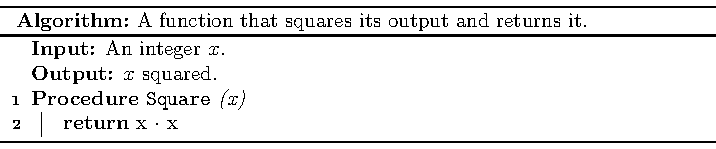
\includegraphics[scale=.95]{assets/chapter4/SquareWithOptions.pdf}
    \caption{An Algorithm2e program, with \texttt{ruled} and \texttt{linesnumbered}.}
    \label{squareWith}
\end{figure}

\begin{figure}[ht]
    \centering
    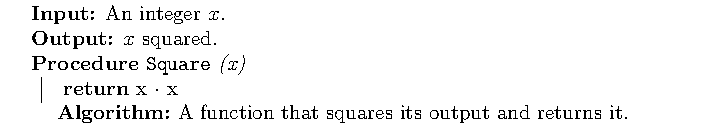
\includegraphics[scale=.95]{assets/chapter4/SquareWithoutOptions.pdf}
    \caption{An Algorithm2e program, without \texttt{ruled} and \texttt{linesnumbered}.}
    \label{squareWithout}
\end{figure}

Lastly, all documents transpiled to TBP include \texttt{\textbackslash DontPrintSemicolon} to prevent lines ending with semicolons, and \texttt{\textbackslash renewcommand\{\textbackslash thealgocf\}\{\}} to avoid numbering the compiled result. All TBP examples so far in this thesis shows the result of including the latter. Since we only transpile the topmost function in a file, we feel like excluding the number looks cleaner. However, if we were to transpile multiple functions, it might make sense to remove it.

\section{Flowchart Writer}

Our third and last writer converts internal representations to LaTeX programs using the TikZ package. Compiling these files produce flowcharts. We believe there is value to working with such a different abstraction level (compared to Gourmet and TBP), and pretty flowcharts helps showcase Psnodig's powerfulness. \\

Just like the TBP writer, the IBP writer only works on topmost function in a file, ignoring the program description, structs and function call. Our reasoning is the same as earlier. \\

\subsection{Compatibility with Psnodig}

To make the corresponding flowcharts clear as well as pleasing, we have opted for three different node themes. This will make it easier to differentiate significant contexts. \\

The start node and all return nodes have the same theme of rectangles with white text on a dark background. Statements containing a list of statements have the same theme of ellipses with black text on a yellow background. Lastly, all remaining statements have the theme of rectangles with black text on a light purple background. \Cref{flowchartColours} shows the result of transpiling a simple function, showcasing all the aforementioned node styles. \\

\begin{figure}[ht]
    \centering
    \includegraphics[scale=.5]{assets/def_FlowchartColours.png}
    \caption{A program showcasing all the different node types the Flowchart generator produces.}
    \label{flowchartColours}
\end{figure}

Just like the TBP writer, the IBP writer uses mathematical notation where appropriate. For instance, \texttt{x \&\& y} is transpiled to \texttt{x $\land$ y}. Contrary to the TBP writer however, Psnodig's library functions are not considered. That means that code like \texttt{length(collection)} will look identical both in the source code and the corresponding flowchart. \\

There are a few design choices worth noting. Return expressions do not explicitly say \texttt{return}, as their context is given by the node theme. Also, recursive function calls do not have an arrow back to the original node stating the function name, but are instead written as their own nodes. For one, there is no straightforward way of creating arrows on this form with TikZ, but we also believe a flowchart with too many arrows looks confusing. \\

All statements are displayed in a simple rectangular box, but \texttt{Loop}-, \texttt{ForEach}-, \texttt{For}-, and \texttt{If}-statements are - as previously mentioned - given their own node themes. This is because they break with the standard linear pattern, and contain statements of their own. \\

\texttt{\textbf{For} identifier from to statements} starts with assigning \\ \texttt{identifier} to \texttt{fromRange}. The next node is a light yellow rectangle. If \texttt{from} and \texttt{to} are both numericals, the rectangles text will be either \texttt{from < to ?} or \texttt{from > to ?}, depending on their values. If they are not both numericals, the default is \texttt{from < to ?} since we do not evaluate expressions, and have no way of knowing their actual values. \\

From this light yellow rectangle, we have an edge labeled \texttt{true} which points to the next statement \textit{after} the current \texttt{\textbf{For}} (if there are any). In the opposite way, an edge labeled \texttt{false} points to the first statement in \texttt{statements}. After the last of these, there is an assignment statement, either incrementing or decrementing \texttt{identifier}, before pointing back to the light yellow rectangle. \\

\Cref{forExample1}, \Cref{forExample2}, and \Cref{forExample3} shows the three different ways a \texttt{\textbf{For}}-statement can be transpiled to a flowchart. \\

\begin{figure}[ht]
    \centering
    \includegraphics[scale=.38]{assets/def_ForExample2.png}
    \caption{A \texttt{For}-statmenet where \texttt{from < to}.}
    \label{forExample1}
\end{figure}

\begin{figure}[ht]
    \centering
    \includegraphics[scale=.38]{assets/def_ForExample3.png}
    \caption{A \texttt{For}-statmenet where \texttt{from > to}.}
    \label{forExample2}
\end{figure}

\begin{figure}[ht!]
    \centering
    \includegraphics[scale=.38]{assets/def_ForExample2.png}
    \caption{A \texttt{For}-statmenet where \texttt{from} and \texttt{to} are not both numericals.}
    \label{forExample3}
\end{figure}

\texttt{\textbf{ForEach} identifier collection statements} starts with a light yellow rectangle asking if we have iterated \texttt{collection}. From here there are two arrows. The first is labeled \texttt{true} and points to the next statement after the current \texttt{\textbf{ForEach}} (if there are any). \\

The other one is labeled \texttt{false} and points to a statement stating \texttt{identifier $\gets$ next element in collection}. Then each statement in \texttt{statements} is presented. After the last of these, there is an arrow pointing back to the light yellow rectangle. A working example is presented in \Cref{flochartForEach}. \\

\begin{figure}[ht]
    \centering
    \includegraphics[scale=0.39]{assets/def_ForEachExample.png}
    \caption{A \texttt{ForEach}-statement, iterating a variable \texttt{teams}.}
    \label{flochartForEach}
\end{figure}

\texttt{\textbf{While} condition statements} largely follows the pattern of \texttt{\textbf{ForEach}}. The statement starts with a light yellow rectangle displaying \texttt{condition} followed by a question mark. \\

There are again two edges: The first is labeled \texttt{true} and points to the next statement after the current \texttt{\textbf{While}} (if there are any). The other is labeled \texttt{false} and points to the first statement in \texttt{statements}. The last of these points back to the light yellow rectangle. A working example is presented in \Cref{flochartWhile}. \\

\begin{figure}[ht]
    \centering
    \includegraphics[scale=0.39]{assets/def_WhileExample.png}
    \caption{A \texttt{While}-statement, iterating until \texttt{i} reaches the value of \texttt{bigNumber}.}
    \label{flochartWhile}
\end{figure}

\texttt{\textbf{If} condition statements else} is the most intricate statement of the four discussed in this section. Again we start with a yellow rectangle displaying \texttt{condition} followed by a question mark. An edge labeled \texttt{true} points to the first statement in \texttt{statements}. Another edge labeled \texttt{false} points to either \texttt{else}, the next statement after the current \texttt{\textbf{If}}, or nothing, since both are optional. \\

If last statement in \texttt{statements} is not a \texttt{Return}-statement, it must point to the next statement outside the current \texttt{\textbf{If}} (if there is one). If \texttt{else} is present, the same applies to its statement list. \\

If the last statement in \texttt{statements} is a \texttt{Return}-statement, and the same is the case for all subsequent \texttt{else}s, the next statement after the current \texttt{\textbf{If}} is unreachable. If our code still has this structure, we are told in the command line, and the transpilation is interrupted. \\

\forsup{Her skal jeg vise en del eksempler}

\subsection{Output}

Transpiling IBP with the command line works precisely like it does with TBP. We run \texttt{psnodig ibp program} to transpile the program and receive a corresponding LaTeX file, given that the program is syntactically correct. If we also wish for the compiled result, we add a \texttt{pdf} flag. \\

\Cref{Example output from compiling Flowchart} shows the (most important parts of the) LaTeX file we receive by transpiling the program in \Cref{Gourmet f}. We see how every node has a unique id, reference a tikzstyle, and how the metadata describes their placement. We also make a point out of drawing all the edges \textit{after} drawing all the nodes, for the sake of readability. To take this one step further, we also sort the edges on the id of the source node. \\

\begin{lstlisting}[caption={Excerpt of the LaTeX from transpiling \Cref{Gourmet f} to IBP.}, captionpos=b, label={Example output from compiling Flowchart}]
\node (0) [startstop] {f()};
\node (1) [statement, below of=0] {v = 5};
\node (2) [startstop, below of=1] {v};

\draw [edge] (0) -- (1);
\draw [edge] (1) -- (2);
\end{lstlisting}
